\documentclass[]{fbmatheblattEWP}
%%%%%%%%%%%%%%%%%%%%%%%%%%%%%%%%%%%%%%%%%%%%%%%%%%%%%%%%%%%%%%%%%%%%%%%%%%%%%%%%
% latex-preamble for exercises: Einführung in das wissenschaftliche Programmieren (EWP), TU Kaiserslautern
% lecturer: Dr. Martin Bracke
% author: Matthias Andres
% email: andres@mathematik.uni-kl.de
% last update: October 20, 2018
%%%%%%%%%%%%%%%%%%%%%%%%%%%%%%%%%%%%%%%%%%%%%%%%%%%%%%%%%%%%%%%%%%%%%%%%%%%%%%%%

\usepackage[]{standalone}
\usepackage[utf8]{inputenc}
\usepackage[]{amsmath}
\usepackage[]{amsfonts}
\usepackage[]{amssymb}
\usepackage[]{amsthm}
\usepackage{bm}
\usepackage[]{eurosym}
\usepackage[]{graphicx}
\usepackage[]{subfig}
\usepackage[]{caption}
\usepackage[]{alltt}
\usepackage[]{colortbl}
\usepackage[]{stmaryrd}
\usepackage[]{enumerate}
\usepackage[]{tikz}
\usepackage[]{pgfplots}
\usepackage{nicefrac}
\usepackage{empheq}
\usepackage{makecell}
\usepackage{listings} % code embedding
\usepackage{enumerate} % change style of enumerate

% bibliography stuff
\usepackage{natbib}
\usepackage{bibentry}
\bibliographystyle{plain}
\nobibliography*

\usepackage{EWPStyle}

\Veranstaltung{ Titel der Vorlesung}

\Dozenten{ Name 1 \\ Name 2} 
\newcommand{\pathToResource}{/home/crack/Uni/exercisesheetmanager/resources}

\begin{document}

\Daten{WS1920, 31.10.2019}{21.11.2019 \\ 12:00 Uhr}{Abgabefrist: \\ \hspace{1em}}{Praktikumsblatt}{1}

\begin{Blatt}{disclaimer}

\begin{Aufgabe}{Iterative Solvers}

\weblink{https://www.uni-kl.de/}{}

\begin{figure}[h!]
	\centering
	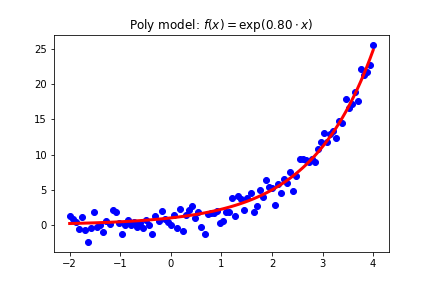
\includegraphics[width=5cm]{\pathToResource /material/modelvsdata.png}
	\bild{Datenpunkte}
\end{figure}
\cite{Dahmen}
\Hinweis{Die Funktionen \codi{surf, fix, cumsum} könnten hilfreich sein.}


\end{Aufgabe}
\begin{Aufgabe}{Gau{\ss}-Filter}

\weblink{https://www.uni-kl.de/}{}

\begin{figure}[h!]
	\centering
	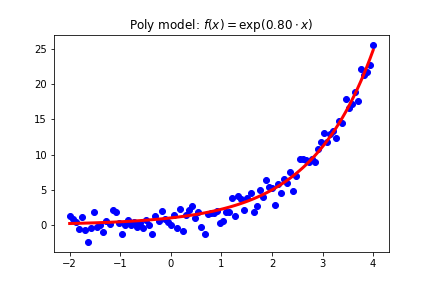
\includegraphics[width=5cm]{\pathToResource /material/modelvsdata.png}
	\bild{Datenpunkte}
\end{figure}
\cite{Dahmen}
\Hinweis{Die Funktionen \codi{surf, fix, cumsum} könnten hilfreich sein.}


\end{Aufgabe}
\begin{HausaufgabeNoDiscussion}{Iterative Solvers}

\weblink{https://www.uni-kl.de/}{}

\begin{figure}[h!]
	\centering
	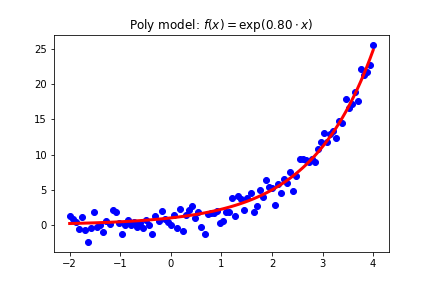
\includegraphics[width=5cm]{\pathToResource /material/modelvsdata.png}
	\bild{Datenpunkte}
\end{figure}
\cite{Dahmen}
\Hinweis{Die Funktionen \codi{surf, fix, cumsum} könnten hilfreich sein.}


\end{HausaufgabeNoDiscussion}
\begin{Hausaufgabe}{Gau{\ss}-Filter}{4 Punkte}

\weblink{https://www.uni-kl.de/}{}

\begin{figure}[h!]
	\centering
	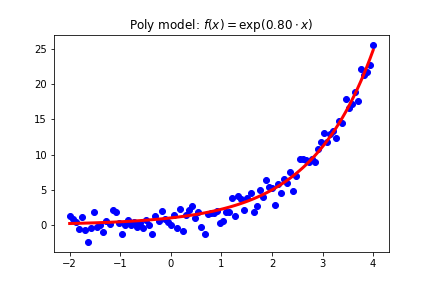
\includegraphics[width=5cm]{\pathToResource /material/modelvsdata.png}
	\bild{Datenpunkte}
\end{figure}
\cite{Dahmen}
\Hinweis{Die Funktionen \codi{surf, fix, cumsum} könnten hilfreich sein.}


\end{Hausaufgabe}


\end{Blatt}

\nobibliography{./literature}

\end{document}